% Created 2018-03-14 Wed 22:28
% Intended LaTeX compiler: pdflatex
\documentclass[pressentation,10pt,aspectratio=1610, xcolor=table]{beamer}
\usepackage[utf8]{inputenc}
\usepackage[T1]{fontenc}
\usepackage{graphicx}
\usepackage{grffile}
\usepackage{longtable}
\usepackage{wrapfig}
\usepackage{rotating}
\usepackage[normalem]{ulem}
\usepackage{amsmath}
\usepackage{textcomp}
\usepackage{amssymb}
\usepackage{capt-of}
\usepackage{hyperref}
\usepackage[french, frenchb]{babel}\usepackage{etex}\usepackage{minted}\usemintedstyle{emacs}\usepackage{pifont}\usepackage{booktabs}\usepackage{pgfplotstable}
\usepackage{tikz}\usepackage{amsmath}\usepackage{pgfplots}\usepackage{etex}\usepackage{mathspec}\usepackage{smartdiagram}\usetikzlibrary{arrows,shapes,positioning,mindmap,decorations.pathreplacing,backgrounds,overlay-beamer-styles,calc,3d,fit}
\defaultfontfeatures{Ligatures=TeX} \usepgfplotslibrary{statistics,ternary,dateplot}\usepackage{appendixnumberbeamer}\usepackage{animate}\pgfplotsset{/pgf/number format/assume math mode=true}
\setmathsfont(Digits,Latin,Greek)[BoldFont=Fira Sans Bold]{Fira Sans Light} \usepackage{pgfplotstable}\usepackage{siunitx}
% Define the layers to draw the diagram
\pgfdeclarelayer{background}
\pgfdeclarelayer{foreground}
\pgfsetlayers{background,main,foreground}
% Define block styles
\tikzstyle{bblock}=[draw, text width=8.0em, text centered,
minimum height=1.8em,drop shadow]
\tikzstyle{datanode} = [bblock, fill=blue!20, text width=8em, minimum width=8em,
minimum height=4em, drop shadow]
\tikzstyle{process} = [bblock, fill=green!20, text width=8em, minimum width=8em,
minimum height=4em, rounded corners, drop shadow]
\tikzstyle{texto} = [above, text width=10em, text centered]
\tikzstyle{linepart} = [draw, thick, color=black!50, -latex', dashed]
\tikzstyle{line} = [draw, thick, color=black!50, -latex']
\tikzstyle{ur}=[draw, text centered, minimum height=0.01em]
\tikzstyle{datanode} = [bblock, fill=blue!20, text width=8em, minimum width=8em,
minimum height=4em, drop shadow]
\tikzstyle{classnode} = [bblock, fill=orange!20, text width=8em, minimum width=8em, minimum height=4em, drop shadow]
% Define distances for bordering
\newcommand{\blockdist}{1.3}
\newcommand{\edgedist}{1.5}
\newcommand{\process}[3]{node (#1) [process]
{\textbf{#2}\\{\scriptsize\textit{#3}}}}
\newcommand{\datanode}[2]{node (#1) [datanode] {\textbf{#2}}}
\newcommand{\bdnode}[2]{node (#1) [bdnode] {\textbf{#2}}}
\newcommand{\classnode}[2]{node (#1) [classnode] {#2}}
% Draw background
\newcommand{\background}[5]{%
\begin{pgfonlayer}{background}
% Left-top corner of the background rectangle
\path (#1.west |- #2.north)+(-0.5,0.5) node (a1) {};
% Right-bottom corner of the background rectanle
\path (#3.east |- #4.south)+(+0.5,-0.25) node (a2) {};
% Draw the background
\path[fill=yellow!20,rounded corners, draw=black!50, dashed]
(a1) rectangle (a2);
\path (a1.east |- a1.south)+(1.25,-0.3) node (u1)[texto]
{\scriptsize\textsc{#5}};
\end{pgfonlayer}}
\usetheme{metropolis}
\usecolortheme[snowy]{owl}
\author{Mathieu Fauvel}
\date{23 mars 2018}
\title{Occupation des sols à l'aide de séries temporelles d'images satellitaires}
\subtitle{27\iemes~ Journées de la Recherche IGN}
\metroset{progressbar=frametitle,numbering=fraction,titleformat=smallcaps,block=fill,sectionpage=simple,subsectionpage=simple}
\setbeamercovered{again covered={\opaqueness<1->{25}}}
\author[Mathieu Fauvel]{Jordi Inglada$^{1}$, Arthur Vincent$^{1}$, Vincent Thieirion$^{1}$ et Mathieu Fauvel$^{1,2}$}
\institute[INRA]{$^{1}$ CESBIO, Université de Toulouse, CNES, CNRS, IRD, UPS, Toulouse, France\\ $^{2}$ DYNAFOR, Université de Toulouse, INRA, Castanet-Tolosan, France}
\setbeamertemplate{footline}
{%
\leavevmode%
\hbox{\begin{beamercolorbox}[wd=.5\paperwidth,ht=2.5ex,dp=1.125ex,leftskip=.3cm plus1fill,rightskip=.3cm]{author in head/foot}%
\usebeamerfont{author in head/foot}\insertshortauthor: \insertshorttitle
\hfill%
\end{beamercolorbox}%
\begin{beamercolorbox}[wd=.5\paperwidth,ht=2.5ex,dp=1.125ex,leftskip=.3cm,rightskip=.3cm plus1fil]{title in head/foot}%
\usebeamerfont{title in head/foot}\hfill\insertframenumber/\inserttotalframenumber\hspace{2em}
\end{beamercolorbox}}%
\vskip0pt%
}
\setbeamertemplate{blocks}[rounded][shadow=false,]
\setbeamersize{text margin left  = 0.5cm}
\setbeamersize{text margin right = 0.5cm}
\setbeamertemplate{itemize item}[square]
\setbeamertemplate{itemize subitem}[triangle]
\setbeamertemplate{itemize subsubitem}{$\star$}
\setbeamertemplate{navigation symbols}{}
\begin{document}

\maketitle
\begin{frame}{Outline}
\tableofcontents
\end{frame}

\section{Occupation et usage des sols par télédétection}
\label{sec:org9394a74}
\begin{frame}[label={sec:org3aabfae}]{Occupation et usage des sols}
\begin{block}{Qu'est ce que c'est ?}
\begin{itemize}
\item Couverture (bio)-physique des terres émergées
\item Utilisation faites par l'homme
\end{itemize}
\end{block}
\begin{block}{Pourquoi ?}
\begin{itemize}
\item Connaître l'état et les tendances d'évolution passées/futures des territoires/paysages
\item Entrée de nombreux travaux de recherche
\end{itemize}
\end{block}
\begin{block}{Comment faire ?}
\begin{itemize}
\item Manuelle,
\item Automatique
\end{itemize}
\end{block}
\begin{block}{Enjeux}
\begin{itemize}
\item Qualité
\item Mise à jours fréquentes \& fraîcheur
\end{itemize}
\end{block}
\end{frame}
\begin{frame}[label={sec:orgabf36f0}]{OCS \& télédétection}
\begin{columns}
\begin{column}{0.5\columnwidth}
\begin{itemize}
\item Classification supervisée des pixels à partir de descripteurs \emph{spatio-spectro-temporel}
$$ f:\mathbf{x} \mapsto z $$
\item Série temporelle \emph{Sentinel-2}
\begin{itemize}
\item Des dizaines de dates
\item Des milliards de pixels
\end{itemize}
\item <2> \textbf{Mais}
\begin{itemize}
\item Bruit dans la donnée (nuages \& ombres)
\item Adéquation STIS \& BD
\item Volume des STIS
\end{itemize}
\end{itemize}
\end{column}
\begin{column}{0.45\columnwidth}
\animategraphics[controls,loop,width=\linewidth]{1}{figures/color_}{1}{17}
\end{column}
\end{columns}
\end{frame}
\begin{frame}[label={sec:org5cbf980}]{CES OSO}
\begin{center}
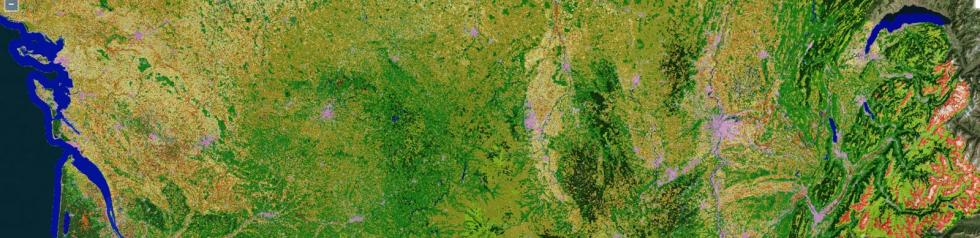
\includegraphics[width=0.8\linewidth]{./figures/imagesat_oso.jpg}
\end{center}

\begin{itemize}
\item Centre d'Expertise Scientifique "CES Occupation des SOls"
\item Caractéristiques, spécifications
\begin{itemize}
\item Production de cartes à échelle nationale:
\begin{itemize}
\item Nomenclature de \textbf{15 à 20 classes},
\item Résolution spatiale entre \textbf{10 m} et 20 m
\item Mise à jour \textbf{annuelle}.
\end{itemize}
\item Données en entrée :
\begin{itemize}
\item STIS (de type Sentinel-2), mais aussi SPOT6, voire Pléiades
\item Des données auxiliaires de référence pour entraînement et validation
\end{itemize}
\end{itemize}
\end{itemize}
\end{frame}

\section{Le produit OSO actuel}
\label{sec:org09e2a6d}
\begin{frame}[label={sec:org2337b5a}]{Caractéristiques}
\begin{itemize}
\item Une cartographie annuelle gratuite et rapidement disponible,
\begin{itemize}
\item Pour la période \og Janvier-Décembre\fg
\item 17 Classes
\item Au format raster ou vecteur (par département)
\item \url{http://osr-cesbio.ups-tlse.fr/\~oso/}
\end{itemize}
\item Une chaîne de traitements \emph{open-source}:
\begin{center}
\url{http://osr-cesbio.ups-tlse.fr/\~oso/posts/2016-02-02-iota2/} 
\end{center}
\item Equipe: \textbf{CESBIO}
\begin{itemize}
\item CIRAD, COSTEL, CNRM, DYNAFOR, ICUBE, ISPA, MATIS \ldots{}
\end{itemize}
\item \emph{Operational High Resolution Land Cover Map Production at the Country
Scale Using Satellite Image  Time Series}.  \(\textsc{Remote Sens.}\)
2017, 9, 95. \url{http://dx.doi.org/10.3390/rs9010095}
\end{itemize}
\end{frame}

\begin{frame}[label={sec:org3a131ee}]{Nomenclature actuelle}
\begin{columns}
\begin{column}{0.5\columnwidth}
\small
\begin{itemize}
\item Surface artificielles
\begin{description}
\item[{CUF}] Continuous urban fabric (CLC 111)
\item[{DUF}] Discontinuous urban fabric (CLC 112)
\item[{ICU}] Industrial or commercial units (CLC 121)
\item[{RSF}] Road surfaces (BD Topo)
\end{description}
\item Surface agricoles
\begin{description}
\item[{ASC}] Annual summer crops (RPG)
\item[{AWC}] Annual winter crops (RPG)
\item[{IGL}] Intensive grassland (RPG)
\item[{ORC}] Orchards (RPG)
\item[{VIN}] Vineyards (RPG)
\end{description}
\end{itemize}
\end{column}
\begin{column}{0.5\columnwidth}
\small
\begin{itemize}
\item Forêts et milieux semi-naturels
\begin{description}
\item[{BLF}] Broad-leaved forest (BD Topo)
\item[{COF}] Coniferous forest (BD Topo)
\item[{NGL}] Natural grasslands (CLC 321)
\item[{WOM}] Woody moorlands (BD Topo)
\end{description}
\item Espaces ouverts avec peu ou pas de végétation
\begin{description}
\item[{BDS}] Beaches, dunes and sand plains (CLC 331)
\item[{BRO}] Bare rock (CLC 332)
\item[{GPS}] Glaciers and perpetual snow (Randolph)
\item[{WAT}] Water bodies (CLC 523 and BD Topo)
\end{description}
\end{itemize}
\end{column}
\end{columns}
\end{frame}

\begin{frame}[label={sec:orgc58e00b}]{OCS France pour 2016}
\begin{center}
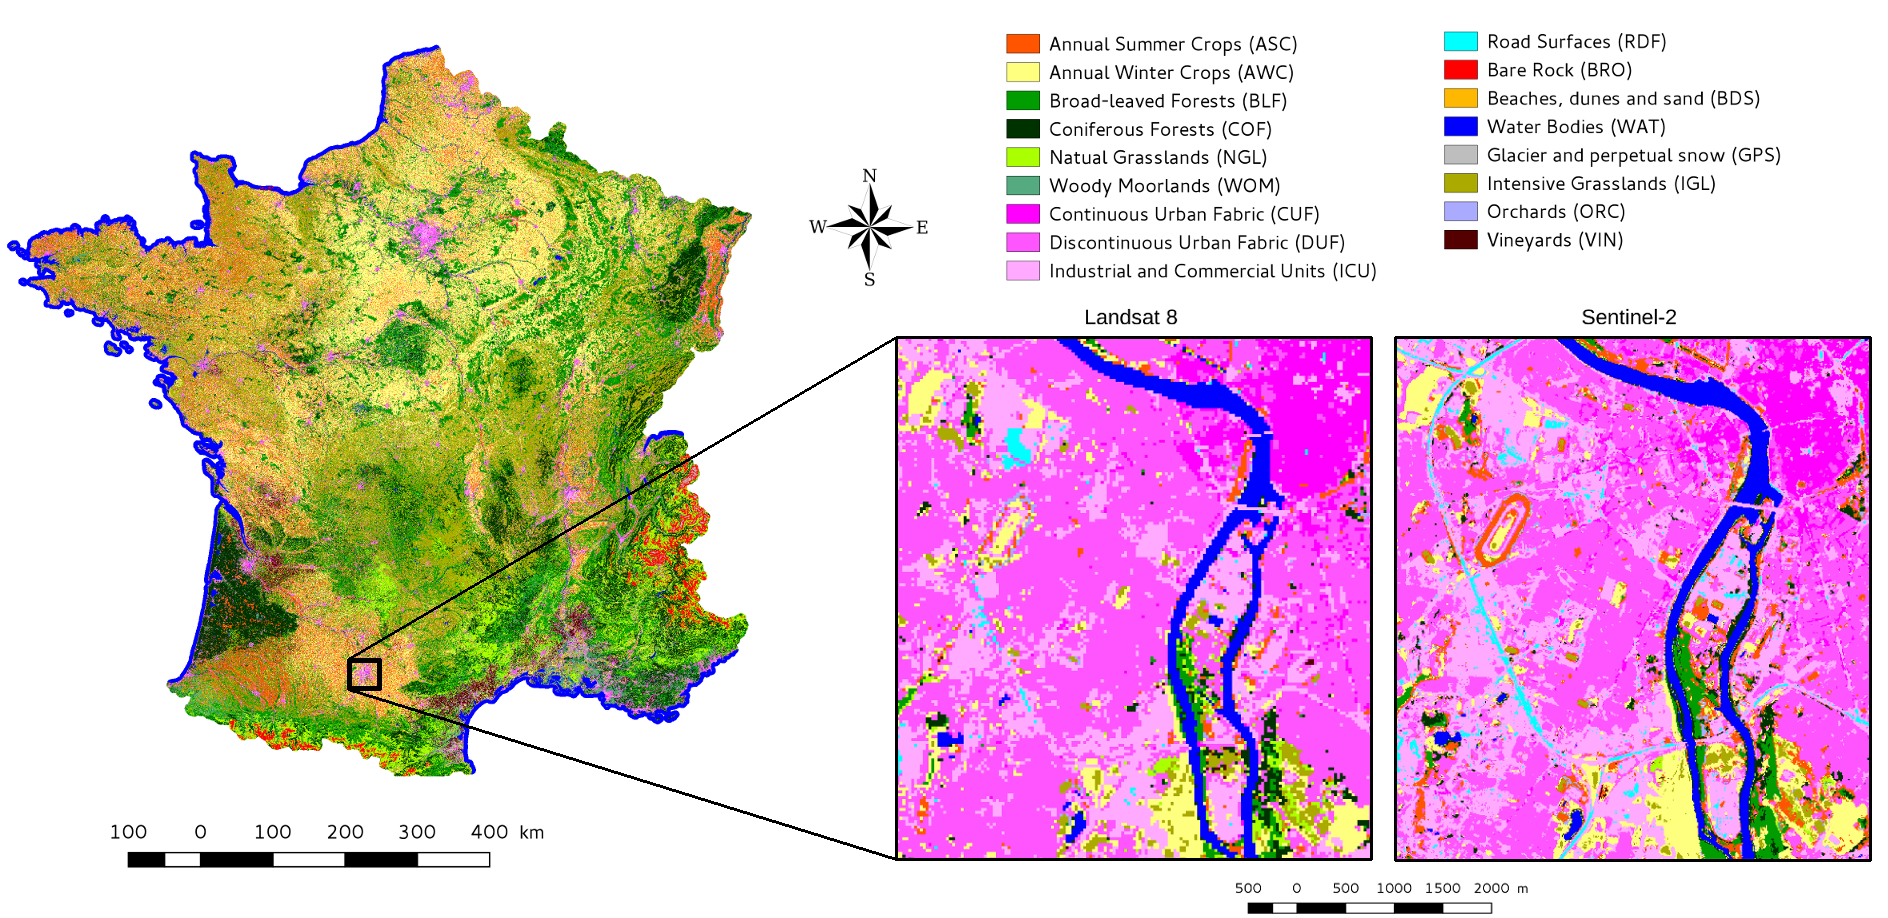
\includegraphics[width=\linewidth]{./figures/OSO_V4.png}
\end{center}
\end{frame}

\begin{frame}[label={sec:org0a681b7}]{Zoom}
\begin{center}
  \only<1>{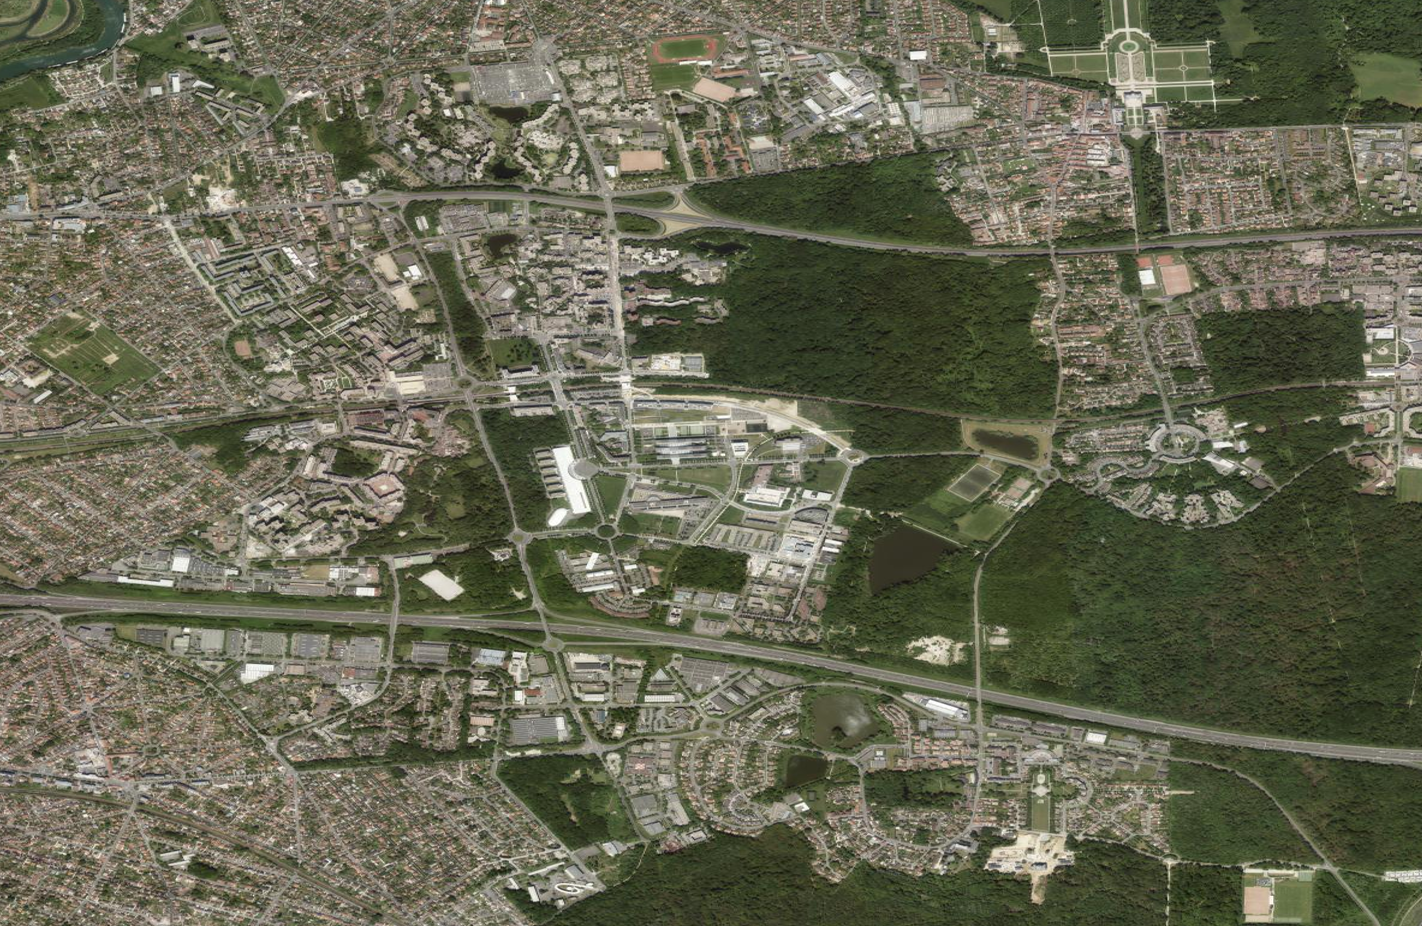
\includegraphics[width=0.8\linewidth]{figures/ensg_ortho.png}}
  \only<2>{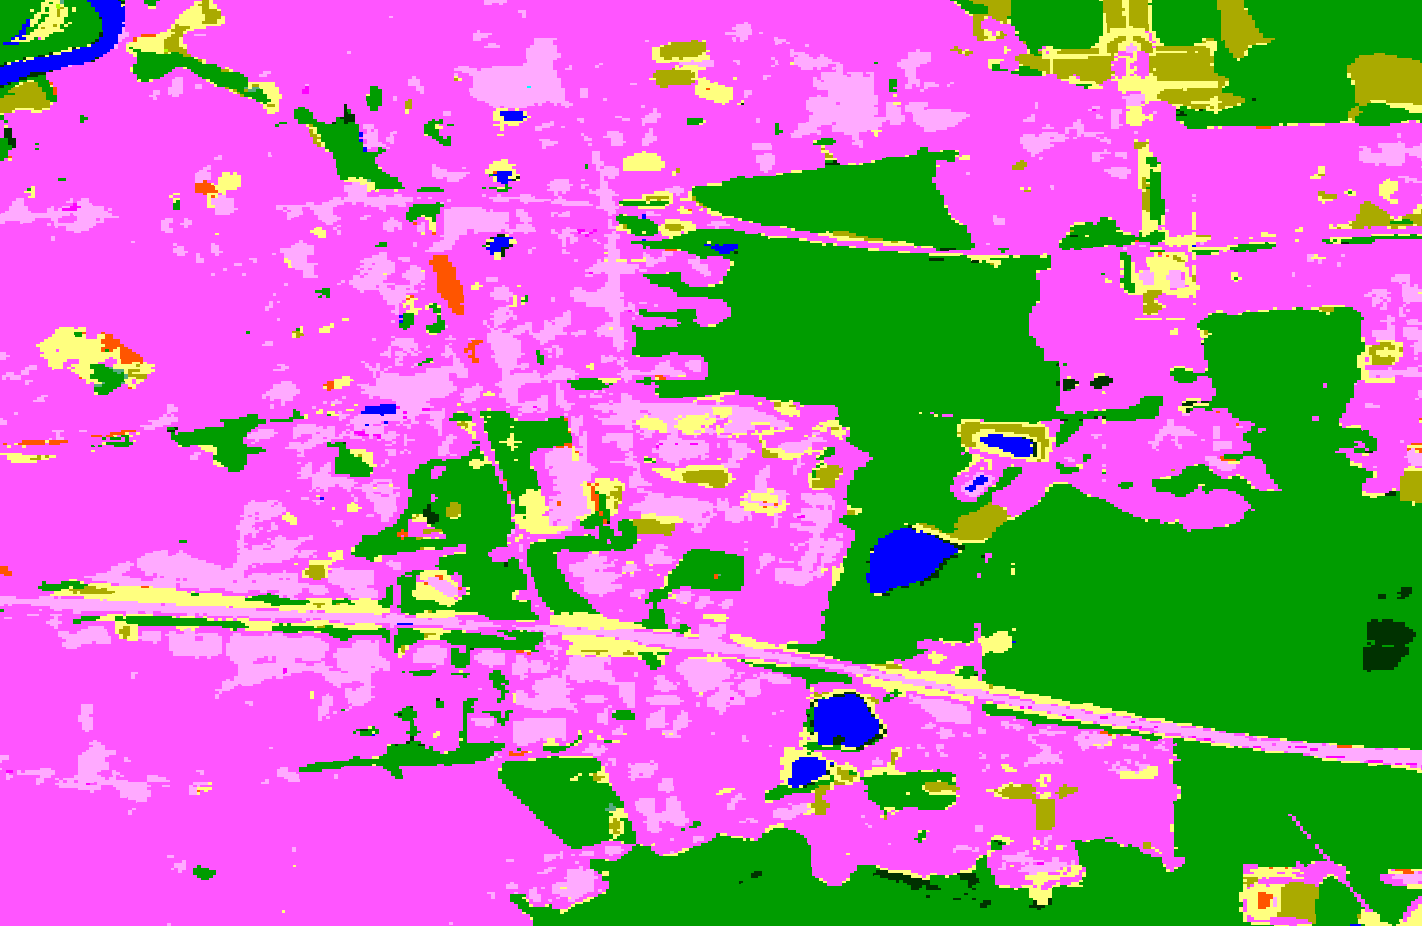
\includegraphics[width=0.8\linewidth]{figures/ensg_oso_10m.png}}
  \only<3>{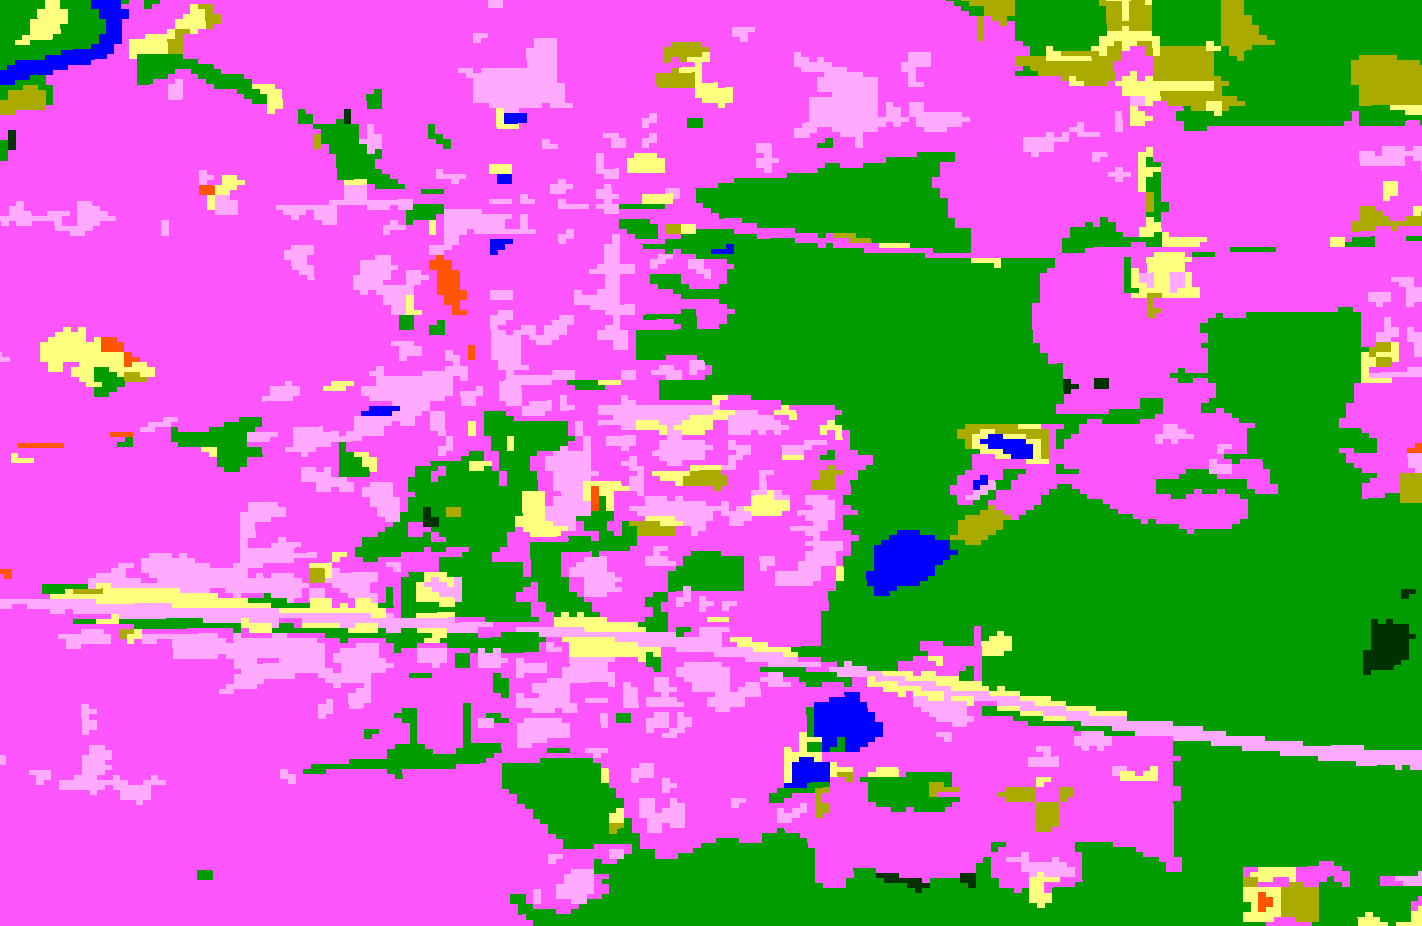
\includegraphics[width=0.8\linewidth]{figures/ensg_oso_20m.png}}
\end{center}
\end{frame}
\begin{frame}[fragile,label={sec:orgf322e1f}]{Précision de classification}
\scriptsize
\pgfplotstableset{
    color cells/.style={
      col sep=comma,
      precision=1, fixed zerofill,
      string type,
      postproc cell content/.code={%
        \pgfkeysalso{@cell content=\rule{0cm}{2.4ex}\cellcolor{black!##1}\pgfmathtruncatemacro\number{##1}\ifnum\number>50\color{white}\fi##1}%
      },
      columns/x/.style={
        column name={},
        postproc cell content/.code={}
      }
    }
}
\begin{center}
\pgfplotstabletypeset[color cells]{
x,ASC,AWC,BLF,COF,NGL,WOM,CUF,DUF,ICU,RSF,BRO,BDS,WAT,GPS,IGL,ORC,VIN
ASC,94,1,0,0,0,0,0,1,0,0,0,0,0,0,1,0,0
AWC,0,98,0,0,0,0,0,0,0,0,0,0,0,0,0,0,0
BLF,0,0,89,5,2,1,0,0,0,0,0,0,0,0,1,0,0
COF,0,0,3,92,1,1,0,0,0,0,0,0,0,0,0,0,0
NGL,0,0,2,5,64,8,0,1,0,0,2,0,0,0,13,0,0
WOM,0,0,5,9,29,41,0,1,0,0,2,0,2,0,5,0,0
CUF,0,0,0,0,0,0,24,46,26,0,0,0,0,0,0,0,0
DUF,0,0,0,1,1,0,0,82,7,0,0,0,0,0,2,0,0
ICU,0,0,0,0,0,0,0,34,58,0,0,0,0,0,1,0,0
RSF,0,0,0,0,0,0,0,19,71,1,0,0,0,0,1,0,0
BRO,0,0,0,0,6,1,0,0,0,0,86,0,0,3,0,0,0
BDS,1,0,2,1,3,5,0,9,8,0,1,43,21,0,1,0,0
WAT,0,0,0,0,0,0,0,0,0,0,0,0,98,0,0,0,0
GPS,0,0,0,0,0,0,0,0,0,0,14,0,0,85,0,0,0
IGL,0,0,1,0,4,0,0,0,0,0,0,0,0,0,90,0,0
ORC,3,2,9,2,7,6,0,8,0,0,0,0,0,0,21,29,7
VIN,5,1,0,1,1,0,0,3,0,0,0,0,0,0,2,0,82
}
\end{center}
\end{frame}
\section{La chaîne de traitements}
\label{sec:orgcd98572}
\begin{frame}[label={sec:orgd47816a}]{Étapes de traitements}
  \begin{center}
    \begin{tikzpicture}[font=\scriptsize, transform shape,scale=0.72]
      \path \datanode{inref}{Reference Data};
      \path (inref.east)+(2.5,0.0) \process{sample}{Sample Selection}{sample\_ratio};
      \path (sample.east)+(2.5,0.0) \datanode{tsamples}{Training Samples};
      \path (sample.east)+(2.5,-1.9) \datanode{vsamples}{Validation Samples};
      \path (inref.south)+(0.0,-2.25) \datanode{valmasks}{Validity Masks};
      \path (valmasks.east)+(2.5,-1.0) \process{interpol}{Linear Interpolation}{t\_0, t\_end, sampling\_period};
      \path (valmasks.south)+(0.0,-1.25) \datanode{inimages}{L2A Input Images};
      \path (interpol.east)+(2.5,0.0) \process{fex}{Feature Extraction}{TOC, NDVI, NDWI, Brightness};
      \path (fex.east)+(3.5,0.0) \process{train}{Training}{nb\_trees, max\_depth, min\_samples};
      \path (train.east)+(2.5,0.0) \datanode{model}{Classification Model};
      \path (interpol.south)+(0.0,-2.5) \process{classif}{Classification}{};
      \path (classif.east)+(2.5,0.0) \datanode{map}{LC Map};
      \path (classif.west)+(-2.5,0.0) \datanode{cropmask}{ROI Mask};
      \path (map.east)+(2.5,0.0) \process{valid}{Validation}{};
      \path (valid.east)+(2.5,0.0) \datanode{stats}{OA, FScore};


      %% arrows
      \path [line] (inref.east) -- node [left] {} (sample);
      \path [line] (sample.east) -- node [left, midway] {} (tsamples);
      \path [line] (sample.east) -- +(0.25,-1.5) -- node [left, midway] {} (vsamples);
      \path [line] (tsamples.east) -- +(3.5,0.0) -- node [above, midway] {} (train);
      \path [line] (vsamples.east) -- +(0.75, 0.0) -- +(0.75, -3.25) -- node [above, midway] {} (valid);
      \path [line] (valmasks.east) -- +(0.25,0.0)-- +(0.25,-0.75)-- node [left] {} (interpol);
      \path [line] (interpol.east) -- node [left] {} (fex);
      \path [line] (fex.east) -- node [left] {} (train);
      \path [line] (train.east) -- node [left] {} (model);
      \path [line] (inimages.east) -- +(0.25,0.00) -- +(0.25,0.75) -- node [left, midway] {} (interpol);
      \path [line] (fex.south) -- +(0.0,-0.75) -- +(-6.25,-0.75) -- +(-6.25,-2.25) -- node [right, midway] {} (classif);
      \path [line] (model.south) -- +(0.0, -1.1) -- +(-12.5, -1.1) -- node [above, midway] {} (classif);
      \path [line] (cropmask.east) -- node [left] {} (classif);
      \path [line] (classif.east) -- node [left] {} (map);
      \path [line] (map.east) -- node [left] {} (valid);
      \path [line] (valid.east) -- node [left] {} (stats);

      % background
      \background{sample}{tsamples}{fex}{fex}{Data Preparation}
      \background{train}{train}{model}{model}{Supervised Learning}
      \background{classif}{classif}{stats}{map}{Map Production}
    \end{tikzpicture}
\end{center}
\end{frame}
\begin{frame}[label={sec:org52bf162}]{Extraction des données d'entraînement/validation}
\begin{onlyenv}<1>
\begin{center}
  \begin{tikzpicture}[font=\scriptsize, scale=0.52, transform shape]
    \path \process{selclass}{Class Selection}{for each source};
    \path (selclass.east)+(2.5,4.5) \datanode{bdtopo}{BD-Topo};
    \path (bdtopo.south)+(0.0,-3.5) \classnode{bdtopoclass}{Broad-leaved forests\\ Coniferous forests\\ Buildings\\ Roads\\ Water};
    \path (bdtopo.east)+(2.5,0.0) \datanode{clc}{CLC};
    \path (clc.south)+(0.0,-3.5) \classnode{clcclass}{Sand, dunes\\ Bare rocks\\ Natural grasslands\\ Oceans and sea\\ Continuous urban\\ Discontinuous urban\\ Industrial and commercial\\ Woody moorlands\\ Water};
    \path (clc.east)+(2.5,0.0) \datanode{rpg}{RPG};
    \path (rpg.south)+(0.0,-3.5) \classnode{rpgclass}{Corn\\Sunflower\\Wheat\\Barley\\Rapeseed\\Cultivated grasslands\\Vineyards\\Olive trees\\Ochards};
    \path (rpg.east)+(2.5,0.0) \datanode{randolph}{Randolph DB};
    \path (randolph.south)+(0.0,-3.5) \classnode{randolphclass}{Glaciers};

    \path (selclass.south)+(0.0,-4.0) \process{checkempty}{Check empty geometries}{};
    \path (checkempty.east)+(2.5,0.0) \process{correctinval}{Correct invalid geometries}{};
    \path (correctinval.east)+(2.5,0.0) \process{removedouble}{Remove double geometries}{};
    \path (removedouble.east)+(2.5,0.0) \process{removeinc}{Remove incorrect geometries}{};
    \path (removeinc.east)+(2.5,0.0) \process{erode}{Negative buffer\\ Remove geometries $<$ 1 pixel}{};


    \path (erode.east)+(2.75,+3) \datanode{bdtopocorr}{BD-Topo selection};
    \path (bdtopocorr.south)+(0.0,-1.0) \datanode{clccorr}{CLC selection};
    \path (clccorr.south)+(0.0,-1.0) \datanode{rpgcorr}{RPG selection};
    \path (rpgcorr.south)+(0,-1.0) \datanode{randolphcorr}{Randolph DB selection};

    \path (clccorr.east)+(3.25,0.0) \process{fusion}{Fusion by difference}{};
    \path (fusion.south)+(0.0,-2.0) \process{removesmall}{Remove geometries $<$ 1 pixel}{};

    \path (removesmall.south)+(0.0,-2.0) \datanode{result}{Final Reference Data};

    \path [line] (2.0, 2.0) -- +(-1.0, 0.0) -- (selclass.north);
    \path [line] (selclass.south) -- node [above] {} (checkempty);
    \path [line] (bdtopo.south) -- node [above] {} (bdtopoclass);
    \path [line] (clc.south) -- node [above] {} (clcclass);
    \path [line] (rpg.south) -- node [above] {} (rpgclass);
    \path [line] (randolph.south) -- node [above] {} (randolphclass);

    \path [line] (checkempty.east) -- node [left] {} (correctinval);
    \path [line] (correctinval.east) -- node [left] {} (removedouble);
    \path [line] (removedouble.east) -- node [left] {} (removeinc);
    \path [line] (removeinc.east) -- node [left] {} (erode);

    \path [line] (erode.east) -- node [above, midway] {} (bdtopocorr.west);
    \path [line] (erode.east) -- node [above, midway] {} (clccorr.west);
    \path [line] (erode.east) -- node [above, midway] {} (rpgcorr.west);
    \path [line] (erode.east) -- node [above, midway] {} (randolphcorr.west);

    \path [line] (bdtopocorr.east) -- node [above] {} (fusion.west);
    \path [line] (clccorr.east) -- node [above] {} (fusion.west);
    \path [line] (rpgcorr.east) -- node [above] {} (fusion.west);
    \path [line] (randolphcorr.east) -- node [above] {} (fusion.west);

    \path [line] (fusion.south) -- node [above] {} (removesmall.north);
    \path [line] (removesmall.south) -- node [above] {} (result.north);

    \background{bdtopo}{bdtopo}{randolphclass}{clcclass}{Reference Data}

  \end{tikzpicture}
\end{center}
\end{onlyenv}
\begin{onlyenv}<2>
\begin{center}
\begin{center}
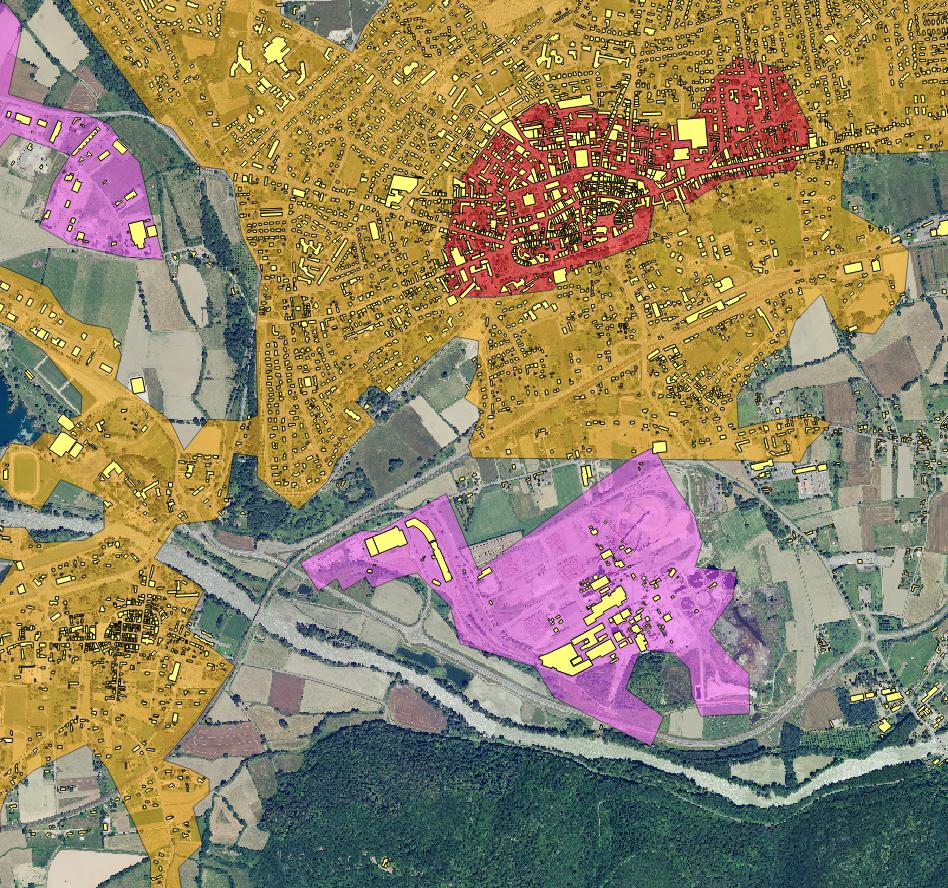
\includegraphics[width=0.55\linewidth]{./figures/BD_ORTHO_CLC_Bati_BDTOPO_All.jpeg}
\end{center}
\end{center}
\end{onlyenv}

\begin{onlyenv}<3>
\begin{center}
\begin{center}
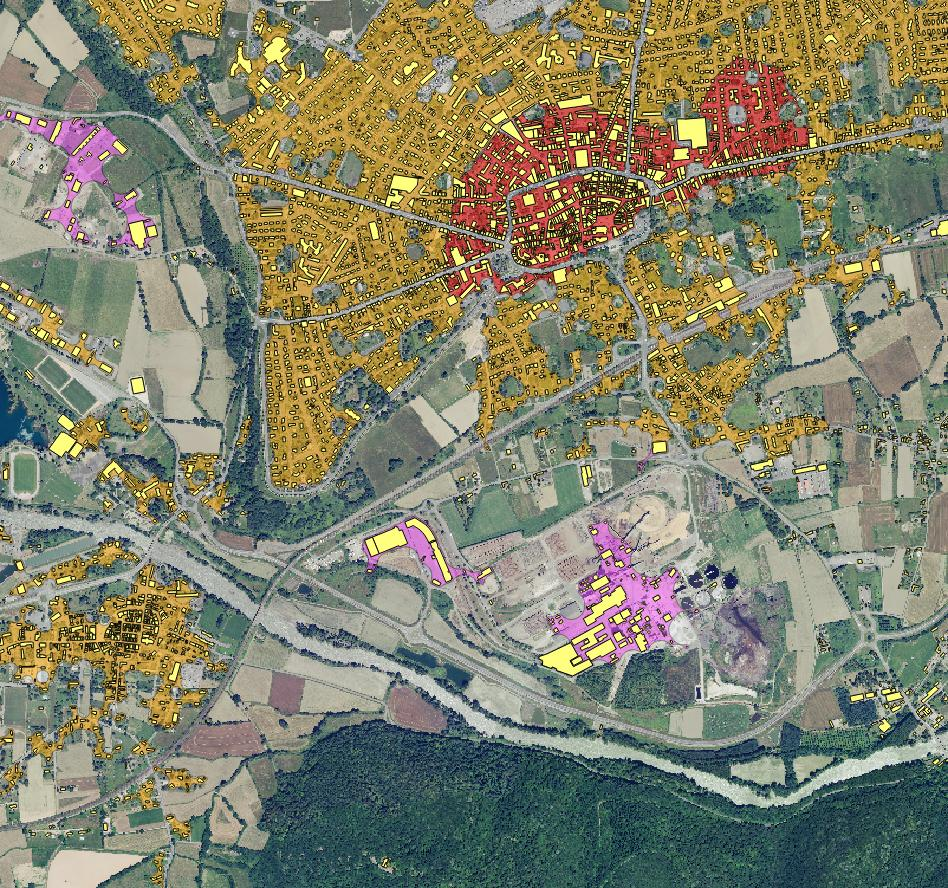
\includegraphics[width=0.55\linewidth]{./figures/BD_ORTHO_ProcessCesbio_BDTOPO_All.jpeg}
\end{center}
\end{center}
\end{onlyenv}
\end{frame}

\begin{frame}[label={sec:org3a5112b}]{Ré-échantillonage temporel}
\begin{onlyenv}<1>
\begin{center}
\begin{center}
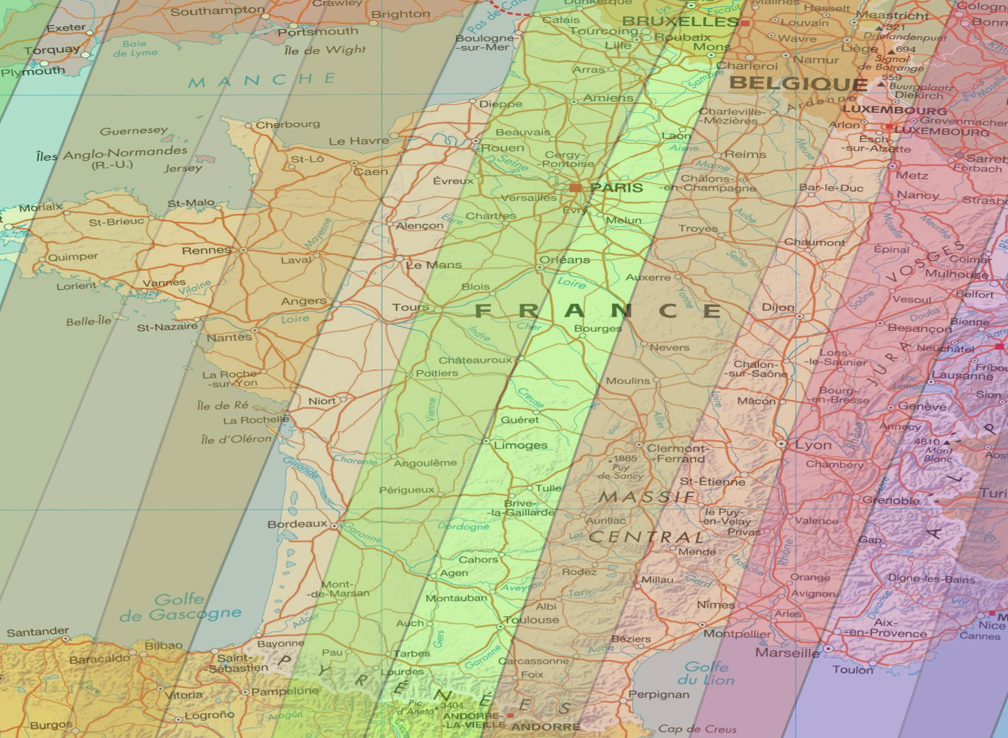
\includegraphics[width=0.725\linewidth]{./figures/S2_tracks.png}
\end{center}
\end{center}
\end{onlyenv}
\begin{onlyenv}<2>
\end{onlyenv}
\end{frame}

\begin{frame}[label={sec:orgace5517}]{Classification}
\begin{columns}
\begin{column}{0.55\columnwidth}
\begin{itemize}
\item Random Forest 
\begin{itemize}
\item Complexité faible
\item Robuste au bruit dans les labels
\item Paramétrisation simple
\end{itemize}
\item Adaptation de domaine
\item Stratification en zones écoclimatiques
\end{itemize}
\end{column}
\begin{column}{0.45\columnwidth}
\begin{center}
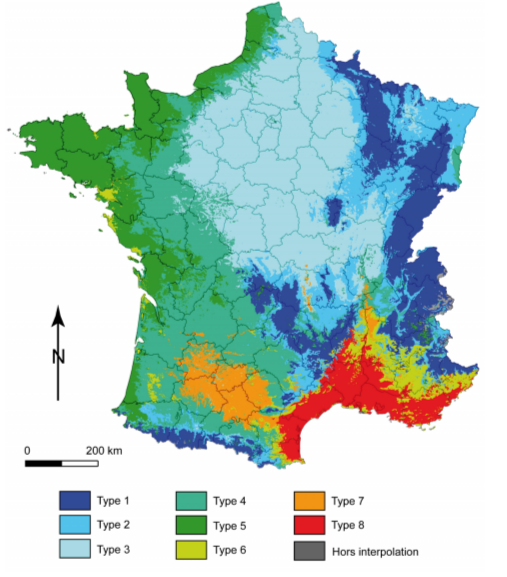
\includegraphics[width=\linewidth]{./figures/climat.png}
\end{center}
\end{column}
\end{columns}
\end{frame}
\end{document}
